\begin{frame}{packet filters = firewalls}
    \begin{itemize}
    \item typical name for packet filter: ``firewall''
    \item especially filtering focused on security
    \end{itemize}
\end{frame}

\begin{frame}<1>[label=ffDesign]{firewall design decisions}
    \begin{itemize}
    \item where to filter?
        \begin{itemize}
        \item typically: \myemph<2>{at ``edges'' of network}
        \item in router, or separate box
        \item can also do elsewhere
        \end{itemize}
    \item how much to track when filtering?
        \begin{itemize}
        \item ``stateless'' or ``stateful''
        \end{itemize}
    \end{itemize}
\end{frame}

\againframe<2>{ffDesign}
\begin{frame}{the corporate firewall}
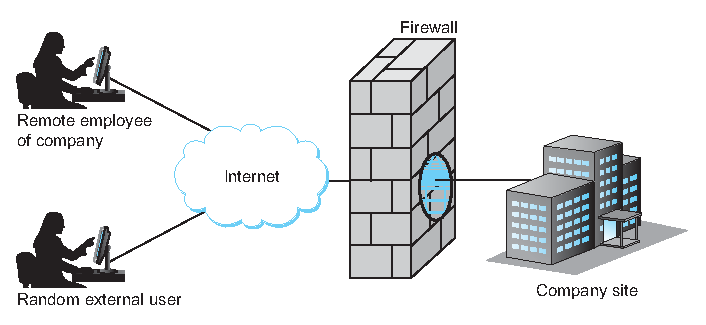
\includegraphics[width=0.9\textwidth]{sysapp-fig214}
\end{frame}

